%%% Time-stamp: <mainrep.tex 19:57, 17 Jul 2016 by P Sunthar>
%%% $Log:$
% This document describes how to use iitbreport style
%********************************************************************

%\documentclass[11pt,a4paper,openright]{report}
\documentclass{iitbreport}

%% Default spacing: 1.5
%% Default font size: 12pt
%% Default font: txfonts (similar to times new roman) 

%% Selectively comment out sections that you want to be left out but
%% maintaining the page numbers and other \ref
\includeonly{%
  intro/introduction,
  related/related_work,
  method/method,
  implementation/implementation,
  results/results,
  conclusion/conclusion,
  dec,abs,pub,ack,images
}

%%% Some commonly used packages (make sure your LaTeX installation
%%% contains these packages, if not ask your senior to help installing
%%% the packages)

\usepackage{booktabs}
\graphicspath{{expt/}}


%%% Macro definitions for Commonly used symbols
\newcommand{\Rey}{\ensuremath{\mathrm{Re}}}
\newcommand{\avg}[1]{\ensuremath{\overline{#1}}}
\newcommand{\tenpow}[1]{\ensuremath{\times 10^{#1}}}
\newcommand{\pder}[2]{\ensuremath{\frac{\partial#1}{\partial#2}}}

% Referencing macros
\newcommand{\Eqref}[1]{Equation~\eqref{#1}}
\newcommand{\Tabref}[1]{Table~\ref{#1}}
\newcommand{\Figref}[1]{Figure~\ref{#1}}
\newcommand{\Appref}[1]{Appendix~\ref{#1}}


\begin{document}
	
%%********************************Frontmatter***********************
% In frontmatter everything comes with roman numbering	
\pagenumbering{roman}
\setcounter{page}{1}

%*******************************************************************
%                         Title Page                            
%*******************************************************************
\title{Training primitive skills to soccer bots}
\subtitle{with the help of Reinforcement Learning}
\author{Rishabh Shah}

%% Print the date. Today's date comes by default, change it here to 
%% other date format, if required:

\date{\today}
% \date{2019}


%% The type of the report can be set here

% \reporttype{A Seminar Report}
%\reporttype{A Thesis}
%\reporttype{A Dissertation}
\reporttype{A B.Tech Technical Project Report}

%% Name of the degree
% \degree{Doctor of Philosophy}
%\degree{Master of Technology}


%% Department/Centre Name
\dept{Department of Computer Science and Engineering}

%% Supervisor and cosupervisor/excosupervisor are not essential parts
%% of a report title page, as it is your report!

%% But if you **have** to put it uncomment these
\supervisor{Shivaram Kalyanakrishnan}
\cosupervisor{Parag Chaudhuri}
%\excosupervisor{External Supervisor}

%% Roll number
\rollnum{150050006}

\maketitle

%*******************************************************************
%                         Copyright Page                          
%******************************************************************* 
% \mycopyright                    

%*******************************************************************
%                         Dedication Page                         
%*******************************************************************
% \dedication[Dedicated to \ldots]        
% \addintoc{Dedication}

%*******************************************************************
%                        Certificate Page                         
%*******************************************************************
%\makecertificate[change title name]{report type} 
%\makecertificate{seminar report} 
%\makecertificate{thesis}
%\makecertificate{dissertation}
%\makecertificate{project report}

%\addintoc{Certificate}

%*******************************************************************
%                         Approval Sheet                         
%*******************************************************************
%\makeapproval{thesis}
%\makeapproval{dissertation}

%*******************************************************************
%                          Declaration                           
%*******************************************************************
% %==================================dec.tex================================
%
\begin{Declaration}
\noindent
I declare that this written submission represents my ideas in my own words and where others' ideas or words have been included, I have adequately cited and referenced the original sources. I declare that I have properly and accurately acknowledged all sources used in the production of this report. I also declare that I have adhered to all principles of academic honesty and integrity and have not misrepresented or fabricated or falsified any idea/data/fact/source in my submission. I understand that any violation of the above will be a cause for disciplinary action by the Institute and can also evoke penal action from the sources which have thus not been properly cited or from whom proper permission has not been taken when needed.

%
%
%
%
%
%
%

\DecSign[\today]



%
\end{Declaration}
%========================================================================
















 
%\addintoc{Declaration}

%******************************************************************
%                          Abstract                             
%******************************************************************  
%============================= abs.tex================================
\begin{Abstract}
\\\\
The research on soccer robot has seen rapid development in recent years. RoboSoccer is focused on training robots to play soccer at a level comparable or even better than humans in the near future. Currently, even the basic skills like balancing, walking and kicking are learned based on mechanical models that need further optimization of skill-specific parameters. Through this project, we explore a generalized method to teach soccer robots these basic skills. Reinforcement Learning's(RL) applications in robotics are of great interest because of their wide applicability. We show that RL can be leveraged to learn some simple skills.  We formulate this problem as RL task where the robot takes actions by adjusting torques to appropriate joints. The rewards experienced are based on pose similarity to motion clips (designed to enact the same skill). Such motion clips provide a model for the robot to follow. The robot then learns to mimic the motion clip while simultaneously trying to balance itself in the simulated world. This is done in two phases namely Retargeting and Training. In Retargeting phase, we try to transfer "motion" from existing motion clips to our RL agent's joint hierarchy. In the Training phase, we train our agent using the data obtained from the retargeted motion clip with the help of a standard RL policy gradient method known as Asynchronous Advantage Actor-Critic (A3C). With extensive testing and tuning, we have been able to successfully train our agent some very primitive skills (both periodic and non-periodic) like hand waves, squats and walking in place. 
\\\\
This report explains the approach taken towards solving this task and the challenges faced in doing so. 
\end{Abstract}
%=======================================================================

                    


%*******************************************************************
%                        Acknowledgements                    
%******************************************************************* 
%%%
\acknowledgments
I would like to express my deepest appreciation and gratitude towards my guides Prof. Shivaram Kalyanakrishnan and Prof. Parag Chaudhuri for providing me with the golden opportunity to work in this field. Their contribution in stimulating suggestions and encouragement have helped me to complete my project and this report.
% \signature{\today}
\signature[Indian Institute of Technology Bombay]{\today}

%========================================================================

%%% Local Variables: 
%%% mode: latex
%%% TeX-master: "../mainrep"
%%% End:  

%******************************************************************
%                         Contents list                         
%******************************************************************
\figurespagefalse
\tablespagefalse
\makecontents % Creats toc, lof, and lot

%******************************************************************
%                        Notations                              
%******************************************************************
\notations[4cm]{List of Symbols}      

%%********************************Mainmatter***********************
% In mainmatter everything comes with arabic numbering	
% \cleardoublepage
\setcounter{page}{1}
\pagenumbering{arabic}

%******************************************************************
%                         Chapters                           
%****************************************************************** 
\hypersetup{hidelinks}
\chapter{Introduction}

\section{RoboCup}
The ultimate goal in AI, probably in robotics, is to build intelligent systems capable of displaying complex behaviors to accomplish the given tasks through interactions with a dynamically changing physical world. RoboCup simulation has emerged as an excellent domain for researchers to test ideas in machine learning and extend the reach of AI. In a generation where machines have evolved to beat humans in the game of Chess and Go, learning in the RoboCup soccer domain involves a whole new set of challenges, such as a continuous multi-dimensional state space, noisy sensors, need to cooperate with other agents to form team strategies and the need to act in real-time. Machine learning techniques have been used in the past on a wide range of tasks in RoboCup that include both individual behaviors and team strategies. We explore one such strategy to learn a generic individual behavior. 
\\\\
Reinforcement learning (RL) is an area of machine learning concerned with how software agents ought to take actions in an environment to maximize some notion of a cumulative reward. In context of RoboCup, we try to explore this idea to train soccer bot to learn basic skills like walking and kicking. The current walk of these bots is somewhat unnatural, and we feel that if it is made more human-like then perhaps robots could learn to perform complex tasks like passing and dribbling much more aptly and therefore get one step closer towards achieving human level competence. To make if more human-like, we model the rewards in our reinforcement learning task in such a way that robots try to mimic human motion while accounting for physical forces that act on it.
\\\\
For good rewards, we need motion clips to be based on our robot hierarchy. A skeleton hierarchy is composed of a series of joints and joints chains with hierarchical relationships. Each joint in a skeleton hierarchy is a child joint and a parent joint. A parent joint is any joint higher in a skeleton's hierarchy than any of the other joints that are influenced by that joint's actions. Standard available motion clips are based on their own specific skeleton hierarchy. Transforming these motion clips to fit on our agent's skeleton hierarchy poses a difficult challenge. Motion retargeting deals with this specific problem on a very generic scale. The objective is to adapt an animated motion from one character to another under some physical constraints. In our case, we have to overcome the issue of different joint lengths while simultaneously constraining correct foot placements. 

\begin{figure}
\centering
  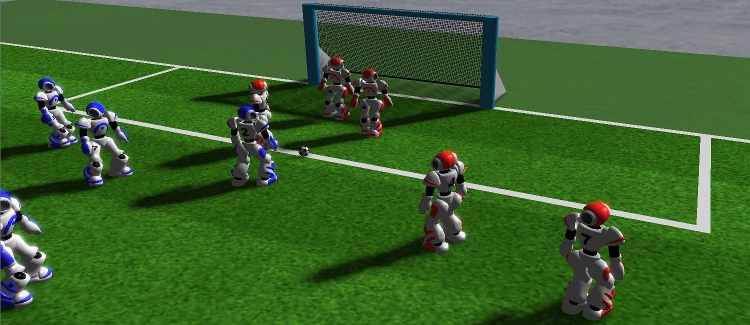
\includegraphics[width=\linewidth]{images/3DRoboCup.jpg}
  \caption{3D RoboCup Simulation with two teams of Red and Blue Nao Agents}
  \label{fig:robocup}
\end{figure}

\section{Problem statement}
Under the standard rules of RoboCup Competition \cite{usermanual}, and physical forces like, friction, gravity and others we need to train a standard Nao agent to walk (and perform other basic skills later) smoothly without falling. This process has to be accomplished via training the soccer bots using human motion clips so that the resultant walk is more natural. This requires agent learning to provide a right set of torques to appropriate joints at right time in the simulation. 

\section{Source Code}
This report along with all the code for this project can be found in \href{https://github.com/rishshah/RoboSoccer}{\underline{this}} Github Link. We have also added a requirements file that contains all the necessary commands needed to setup this project as well as install its dependencies.


\newpage

\begin{figure}
\centering
  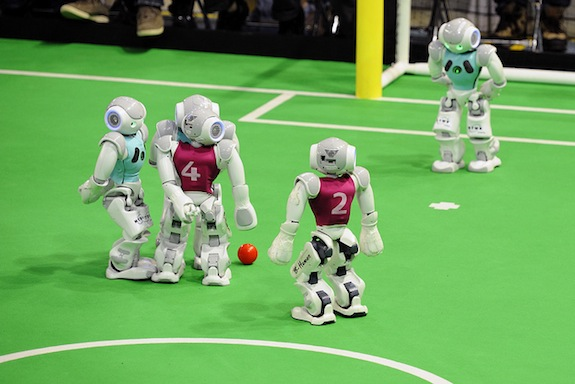
\includegraphics[width=\linewidth]{images/3DRoboCup2.jpg}
  \caption{Real life 3D RoboCup competition between two teams of Red and Blue Nao Agents}
  \label{fig:robocup2}
\end{figure}

\section {Work Partition}
In part 1 of this project, we had designed the general framework for training, getting rewards, running simulations that essentially enabled us to do testing and experimentation in part 2. The retargeting problem as well as other major server flaws were debugged in part 2. All the clips have been trained in this stage.

\section{Report Outline}
The rest of this report is organized as follows. In Chapter 2 we outline the existing literature related to our work. Chapter 3 describes the approaches we tried along with the challenges we faced. In Chapter 4 we provide an overview of our implementation framework. We present our results in Chapter 5 followed by conclusion and future extensions in Chapter 6.
\chapter{Related Work}

Numerous methods have been explored for training agents to walk using RL. Since our work involves a mix of animation and learning to train agents we focus on most closely related work in motion retargeting and RL.

\section{Training Physics Based Models}
[MacAlpine et al. 2012]\cite{AAAI12-MacAlpine} designed architecture for an omnidirectional walk to be used by a humanoid robot soccer agent acting in the RoboCup3D simulation environment. The walk is based on a double linear inverted pendulum model. Their walk engine chooses trajectory such that center of mass of the model swings over the stance foot. After finalizing the position of end effectors via this method, they use inverse kinematics to get positions for rest of the joints and use standard PD controller to calculate the low level torques to be applied to make the bot reach those joint orientations. This is a typical example of using physics-based models that rely on compact set of parameters tuned in order to achieve desired behaviors. The walk though effective, results in unnatural gaits. Also, this method cannot be extended to train robots other kind of complex skills without relying on human insight to implement task-specific strategies. Consequently, we explore RL approach to try to make the walk more human-like as well as to build a generic framework to teach various skills to soccer robot. The RL approach can also be more powerful in learning complex skills easily without much manual parameter tuning. 

\section{Reinforcement Learning}
The introduction of deep neural network models for Reinforcement Learning has given rise to simulated agents that can perform a diverse array of challenging tasks. It offers one of the most general framework to take traditional robotics towards true autonomy and versatility. However, applying RL to high dimensional movement
systems like humanoid robots remains a challenging problem. [Peters et al. 2003]\cite{peters2003reinforcement} discuss merits of various approaches for use of RL in robotics. Policy gradient methods have emerged as an algorithm of choice for many continuous control problems [Sutton et al. 1998]\cite{Sutton:1998:IRL:551283}. However, the resulting behavior learnt through these methods appears less natural than their more manually engineered counterparts. One of the possible reasons is the difficulty in specifying reward functions for a natural movement. Crafting reward functions tailored to specific simulation task requires a substantial degree of human insight. [Xue Bin Peng et al. 2018]\cite{Peng:2018:DED:3197517.3201311} came up with innovative solution to integrate human motion clip data with the reward function for RL agent. Giving higher rewards for mimicking the human motion clip makes the policy/behavior learnt by agent more natural (human-like). We try to adapt this idea to our soccer framework to recreate the results obtained by [Xue Bin Peng et al. 2018]\cite{Peng:2018:DED:3197517.3201311} on our robot hierarchy. 

\section{Maintaining Balance and Stability}
Many skills (like squats and walking) require robot to learn to balance properly throughout the simulation. For Nao \cite{usermanual} robot, this in itself a challenging task. [Tutsoy et al. 2017]\cite{tutsoy2017learning} have tried RL approach along with complete symbolic inverse kinematics just to balance the full lower body of Nao agent. We incorporate some of their ideas in our RL task formulation just to make sure that robot learns to both imitate the motion and maintain its balance without falling. [Xiaochen et al. 2017]\cite{laisurvey} introduced standard stability criteria and provided some common balance strategies. We try to incorporate some of these conditions while designing our reward function. [Yang et al. 2017] \cite{yang2017emergence} also tried to make use of deep RL strategies to learn specific small joint movements on humanoid robots like active push-off of ankles and maintaining the center of mass inside the support polygon to ensure stability. We use some of their ideas to design state space and reward functions to ensure balance.       

\section{Motion Retargeting}
For tailoring motion clips to our bot's skeleton hierarchy we need to solve problem of Motion retargeting. It is essentially transfer of motion (i.e. joint orientations for all frames) from one character hierarchy to another. [Gleicher et al. 1998]\cite{Gleicher:1998:RMN:280814.280820} presents a technique for retargeting motion focusing primarily on adapting the motion of one figure to another with identical structure but different segment lengths. The algorithm is not just to naively copying the angles from one joint to other but also to use inverse kinematics to satisfy end effector constraints. Most other retargeting approaches model constraints to make sure the final animated clip looks natural and similar to original. [Al Borno et al. 2018] \cite{al2018robust} explores the space of robust physics based motion retargeting. They optimize a physical model to approximate an old observed trajectory for the new skeleton.  
\chapter{Our Approach}

\section{Overview}
We divide our work into two phases - Retargeting and Training Phase.
In Retargeting Phase we try to create a suitable motion clip for our RL agent to mimic.
In Training phase, we train our RL agent using the data obtained from the motion clip from previous phase.
\begin{figure}
\centering
  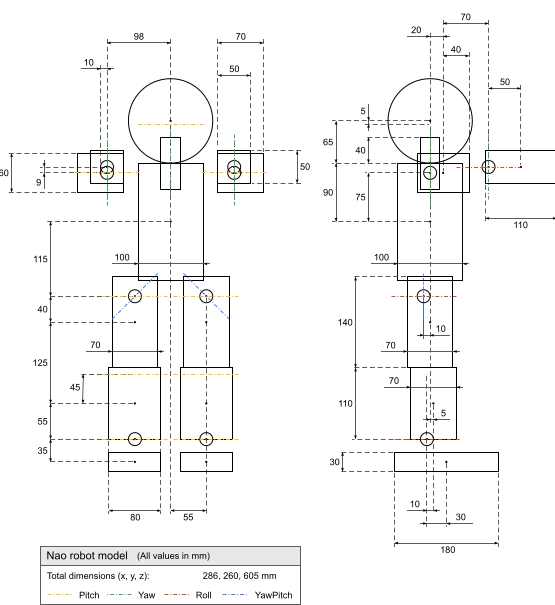
\includegraphics[width=0.7\linewidth, height=10cm,keepaspectratio]{images/nao_param.png}
  \caption{Standard Nao Agent Blueprint used in RoboCup Simulation from Simpspark specifications}
  \label{fig:nao_params}
\end{figure}

\begin{figure}
\centering
  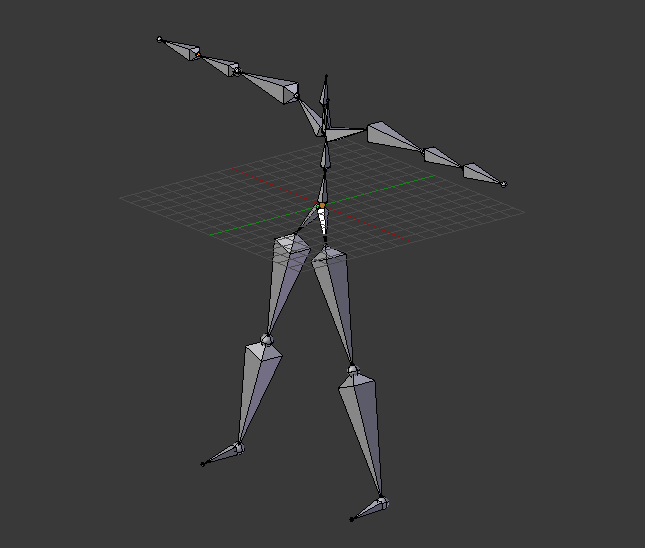
\includegraphics[width=0.7\linewidth, height=10cm,keepaspectratio]{images/mocap_hierarchy.png}
  \caption{Hierarchy of motion clip from walk in place clip before retargeting}
  \label{fig:mocap_hierarchy}
\end{figure}

\section{Retargeting Phase}
	We refer to our robot's hierarchy as \texttt{nao\_hierarchy} and motion clip's bvh hierarchy as \texttt{mocap\_hierarchy}.
	


  \begin{figure}[!b]
  \centering
    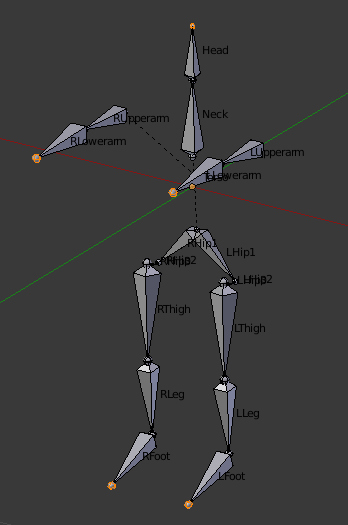
\includegraphics[width=0.7\linewidth, height=10cm,keepaspectratio]{images/nao_hierarchy.png}
    \caption{Blender view of Nao Agent Hierarchy constructed from specifications from Simspark sever and axis restrictions}
    \label{fig:nao_hierarchy}
  \end{figure}
	
  \subsection{Tools}
  We chose to use Blender as our primary BVH tool due to its easier visualization and modeling interface for creating both the \texttt{nao\_hierarchy} and animation. However, some of Blender's inherent flaws in visualizing local pose orientation made it hard to debug the retargeting process. Nevertheless, due to unavailability of other BVH debugging tools, we had to use blender for most of our processing.

	\subsection{Challenges}
	As we can see from Fig \ref{fig:mocap_hierarchy} and Fig \ref{fig:nao_hierarchy}, both the bone lengths and number of joints are different in the \texttt{nao\_hierarchy} compared to the \texttt{mocap\_hierarchy}. Thus, to use the motion clip for our purposes we had to retarget the motion clip to our \texttt{nao\_hierarchy}. This was a non-trivial task involving unforeseen challenges. 
	Firstly, Nao agent has different sets of restrictions on maximum and minimum angles at each hinge joint. Therefore, not all motions could be retargeted to \texttt{nao\_hierarchy}. Moreover, the hip joint in Nao agent has its axis aligned 45 degrees to standard axes and the complementary left and right hip joints are restricted to have same local rotations as seen in Fig \ref{fig:nao_joints}, which makes it harder to retarget any motion using any available tools online. Also, Nao agent has lesser degrees of freedom in almost all joints as compared to the \texttt{mocap\_hierarchy}. Therefore, retargeting problem for \texttt{nao\_hierarchy} was not easy to solve. Thus, to remove dependencies between the two phases, we manually crafted some easy motions like squats and hand wave for debugging training phase so that none of the retargeting errors are responsible for failure in training phase.

	\subsection{Method}
	We manually created a hierarchy in BVH(BioVision Hierarchical data) \cite{Maddock_motioncapture} format  for our Nao \cite{usermanual} agent (which we have referred to as \texttt{nao\_hierarchy}) using the specifications from manual as can be seen from Fig \ref{fig:nao_params}. 

	\\
	Thereafter, we gathered motion clip data from various sources like \href{http://mocap.cs.cmu.edu}{CMU} and work of [Chris Hecker et al. 2008]\cite{sporeanim} and finally chose two simple enough clips that would be easier for agent to learn. First clip described a walk in place motion where in the agent just lifts its legs one by one trying to balance itself. Second clip was a simple hand wave motion. The motion clip originally was made for a skeleton way different than Nao's architecture as seen in Fig \ref{fig:mocap_hierarchy} (which we have referred to as \texttt{mocap\_hierarchy}).
	
	\begin{figure}
	\centering
	  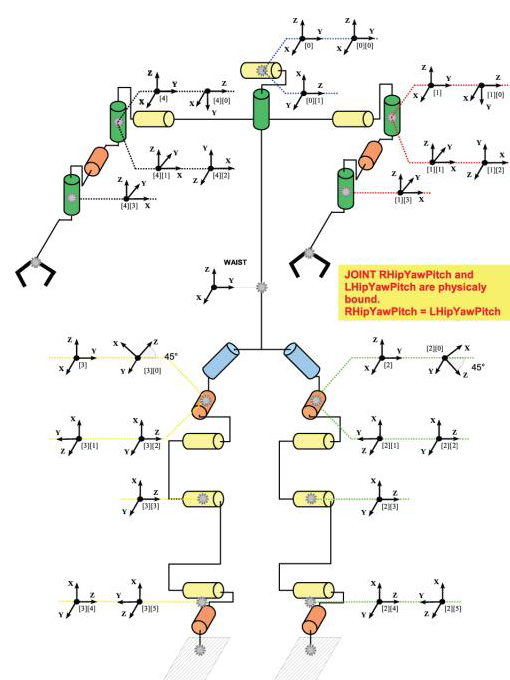
\includegraphics[width=0.7\linewidth, height=10cm,keepaspectratio]{images/nao_joints.png}
	  \caption{Nao parameters indication constraints and axis alignments for all joints}
	  \label{fig:nao_joints}
	\end{figure}

	After taking ideas from the approach of retargeting manually from [Gleicher et al. 1998]\cite{Gleicher:1998:RMN:280814.280820} we devised a mechanism to retarget any generic motion onto our \texttt{nao\_hierarchy}. This involves firstly mapping all joints in \texttt{nao\_hierarchy} to some unique joint in \texttt{mocap\_hierarchy}. Now endpoint of these joints would serve as target positions for our animation to achieve. In second step, we adjust the rest pose (where all the local joint angles are 0) and copy all rotations for every frame of motion clip from \texttt{mocap\_hierarchy} to \texttt{nao\_hierarchy}. 
	Finally, we adjust global target positions of every \texttt{mocap\_hierarchy} joint for the difference in bone lengths and use standard jacobian full body inverse kinematics solver to fine tune the local rotations to make sure corresponding joints of \texttt{nao\_hierarchy} reach the respective target positions in appropriate frames. Some manual tuning was involved to make sure the final animation didn't have sudden large changes in rotations across adjacent frames.
	To tackle the issue of lesser degrees of freedom in our Nao agent, we convert local retargeted rotations into Euler angles, take the required components and discard the remaining ones. This means that its possible that even though the retargeted motion looks good on unconstrained \texttt{nao\_hierarchy} but might not work after removing some specific channels. We made tweaks to rest pose and IK (Inverse Kinematics) parameters to ensure this did not happen for the motion clips we decided to retarget. 
  
\newpage

\section{Training Phase} 
Now to train the agent, we resorted to policy gradient methods due to their proven advantages in domain of continuous action and state spaces. We used the renowned method of Asynchronous Advantage Actor Critic \cite{mnih2016asynchronous} to train our agent.

\subsection{States and Actions}
In our case the action space consists of the angular velocity values of 22 joints (4 on each arm, 6 in each leg, 2 for head and neck as can be seen in Fig \ref{fig:nao_joints}) of the agent. For state space, initially we just used these 22 joints' orientation in degrees, but robot was not even able to learn simple motion clips like hand waves. Applying ideas from  [Yang et al. 2017] \cite{yang2017emergence} we included various other features in our state. These include, the gyrometer values, accelerometer values, height of pelvis from the ground. For learning not to make quick movements we also had to provide input individual joint linear velocities as input to our state. Finally, to learn to periodically repeat motions, we included time as another parameter so that by only resetting time at the end of motion we can make the bot perform periodic motions. We also normalized these inputs by using empirical maximum and minimum values as seen in various simulations. The state space now consisting of more than 50 values can be seen in Fig \ref{fig:neural_net}   

\subsection{Rewards}
Since our motion clips don't involve agent moving forward or any major changes in position of the robot over time, we had to worry about only two kinds of reward functions. First one is \textit{imitation reward} that makes sure that our agent mimics the motion clip to its best extent. Second one is \textit{balance reward} that is specifically purposed to make sure our agent doesn't fall down/lose balance while performing these complicated skills.

\subsubsection{Imitation Reward}
Given the current time in the simulation, we found the corresponding pose in the motion clip. By pose, we mean a tuple consisting of orientation of all 22 joints in the \texttt{nao\_hierarchy}. This pose was used to calculate a similarity metric between current state of and the desired pose in the motion clip. We experimented with various reward functions for capturing the similarity of our agent's pose and target pose of motion clip. Firstly we tried negative of the euclidean distance between the two joint orientation vectors as the similarity metric as it captures the essence of robot's deviation from its current expected pose. 
$$R_{imitation} = - \sum_{i=1}^{22} (n_i - w_i)^2$$
\texttt{where $n_i$ is the ith joint orientation in nao agent pose in degrees \\
and $w_i$ is the ith joint orientation in motion clip pose in degrees}
\vspace{1em}
\\
This wasn't working very well with the A3C algorithm as the learning curve suddenly dropped after 20-30k iterations leading to poorly trained model. After further experiments we found another function of the euclidean distance to stablilize the learning process. 
$$R_{imitation} = e^{- \sum_{i=1}^{22} (n_i - w_i)^2}$$
\texttt{where $n_i$ is the ith joint orientation in nao agent pose in degrees \\
and $w_i$ is the ith joint orientation in motion clip pose in degrees} 
\vspace{1em}
\\
\subsubsection{Balancing Reward}
We experimented with various strategies for this reward too. One way we tried was to check if the agent is about to fall or is already down. This involved tuning falling condition threshold by using accelerometer data from the agent. We then terminated the episode with large negative reward whenever this happened.  \\

$$R_{balance} =
    \begin{cases*}
      -k & if \ \ agent fallen \\ 
       \ 0  & otherwise
    \end{cases*}
$$
\texttt{where $k$ is a large positive constant}
\vspace{1em}
\\
This was not working well due to the fact that agent learnt to "almost" fall at the end of motion clip losing stability way too soon getting overall high rewards. So, to make sure agent never ever loses stability we used  a reward corresponding to maintaining pelvis height from ground above certain level and keeping gyrometer values below some empirical threshold. Using this reward we found that agent doesn't learn to fall but tries to maintain stability throughout the simulation.
$$R_{balance1} =
    \begin{cases*}
        k1 & if \ \ |gyr| < t1 \\ 
       \ 0  & otherwise
    \end{cases*}
$$
$$R_{balance2} =
    \begin{cases*}
        e^{\frac{1}{h}} & if \ \ h > t2 \\ 
       \ 0  & otherwise
    \end{cases*}
$$
\texttt{where $k1$ is a small positive reward in case the gyrometer values ($gyr$) are less than a threshold ($t1$)\\
and  $h$ is the height of pelvis from the ground \\
and $t2$ is another threshold for the height}
\newpage
Finally the total reward at the end of one action step is as following

$$R_{total} = a \times R_{imitiation} + b \times R_{balance1} + c \times R_{balance2}$$
\texttt{where $a,b,c$ are weights tuned empirically for each of the three different rewards)}
\vspace{1em}
\\
\begin{figure}
\centering
  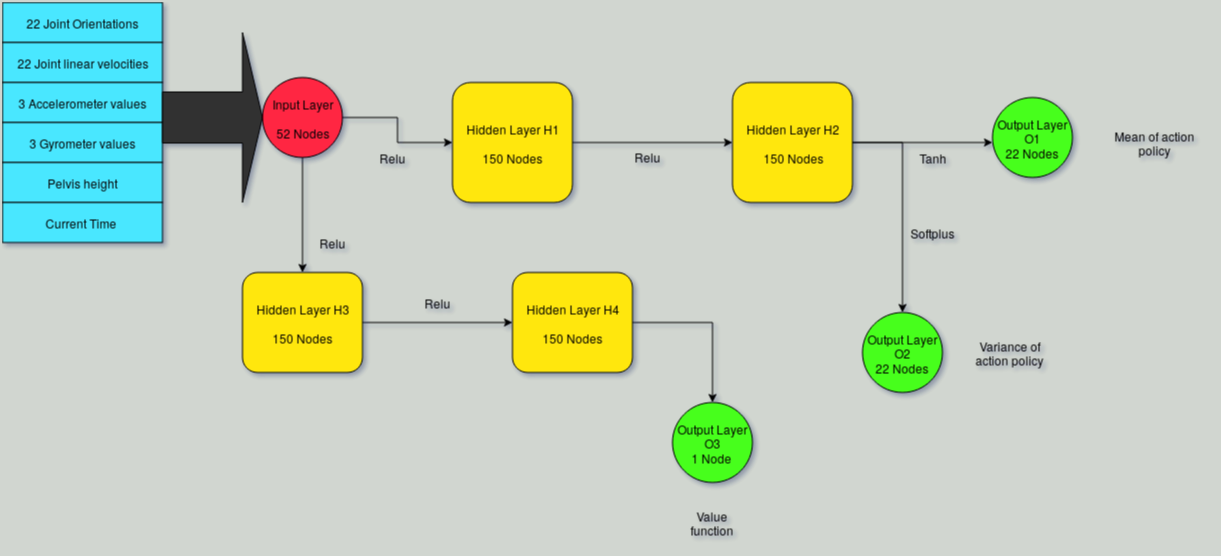
\includegraphics[width=1\linewidth, height=15cm,keepaspectratio]{images/neural_net.png}
  \caption{Neural Network architecture for design used to train robot via A3C.}
  \label{fig:neural_net}
\end{figure}

\subsection{Neural Net}
As with other parameters of this phase we tried various architectures for neural network. Finally, we settled for an architecture where policy was modeled by two neural networks sharing two hidden layers to model mean and variance of policy (actor network). We used an independent additional network for computing value function (critic network). The two hidden layers enable the robot to learn even complex actions for every joint. 
The number of nodes in hidden network was experimented with, and we found that since the state space is large, models trained with around 150 nodes in each hidden layer are good enough to mimic the motions to great accuracies.

Regarding activations of each layer, we found sigmoid and tanh activations to not give results give good results in comparison to Relu activations due to dampened gradients and slow overall learning. Also, we constrained the mean of the policy to be less than a threshold as large torques can have undesirable effects on other joint angle values. 
\chapter{Implementation}

\section{Libraries Used}
We chose Python as our primary language due to its fantastic machine learning support. PyTorch libraries provided excellent API for working with neural nets. The code involves 2 parts. One is the client(agent that is updating its neural net) and other is the environment that client is interacting with. Here the environment encapsulates the simspark server which actually executes actions and returns new state for the agent and runs the whole simulation. Many minor techniques of getting right acceleration values and checking if robot has fallen were obtained from repository of UT Austin Villa's code \cite{utaustin}. 

\section{Server Client Communication} 
Python Simspark agent \cite{pysimspark} was used to communicate with the simspark server. All communication between python-agent and simspark server was relayed through Environment class. We designed its interface similar to python open AI Gym environments. So we abstracted our reward calculation and implementation of features so that the agent could get the next state, reward and boolean flag for termination of episode from  a \texttt{step(action)} function. This takes action as input and gives the above mentioned outputs after performing one step in simulation. This is equivalent to performing a transition in the MDP \cite{Sutton:1998:IRL:551283} for this problem. After every episode, we reset the agent connection to start over. 
\\\\
We faced a lot of problems with this server environment. Since simspark server development is still under progress, it crashes if multiple connections are made and therefore, we have coded a robust environment handling all server side errors and subtly making A3C agent discard the given episode and restart whenever connection between server and client fails abruptly. Another bug in the server was the fact that instead of providing with the next state it gave the current state as the output at every time step. To handle this, we introduced a dummy 0 action between every two consequetive actions sent by the agent. This was meant to do nothing but get next state for the current action. Another issue with this server was the initial position of robot. Instead of being in rest pose on ground, the server initialized the agent in a free fall state. The agent landed on the ground and stabilized in about 1.2 seconds. Such errors took a lot of time to debug due to lack of proper documentation for simspark. Moreover, corrupting the input data this could have been the reason for our initial failures. 

\section{Getting rewards and next state}
Server provided most of the information to generate rewards and next state. The essentials things we received were orientations of 22 joints, our local position, accelerometer and gyrometer values. The rest of the state variables were calculated in the Environment class and abstracted out to the client.

\begin{figure}
\centering
  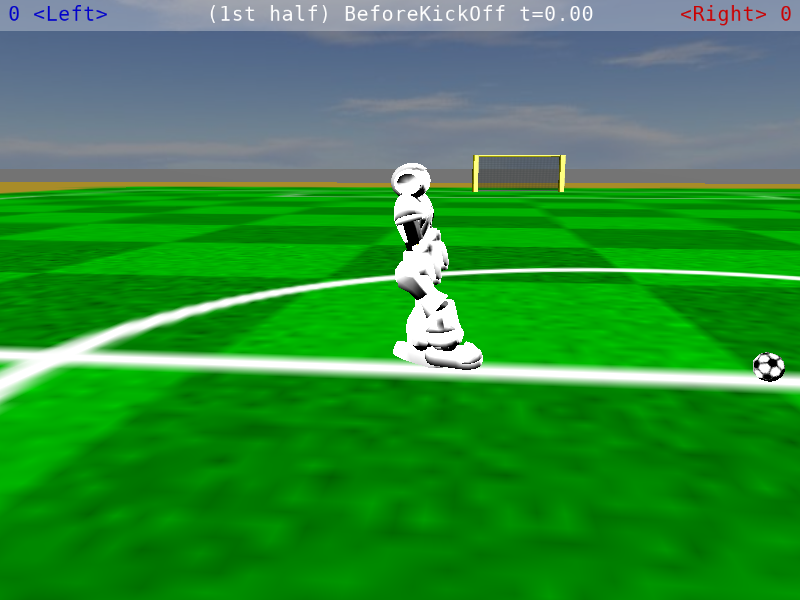
\includegraphics[width=0.5\linewidth, height=6cm,keepaspectratio]{images/monitor.png}
  \caption{Visualization of learning of robot using A3C on a standard Simspark Monitor}
  \label{fig:simulator}
\end{figure}

\section{Initial Pose and Rendering}
For retargeted motion, we had to use almost 50-100 frames to get to the initial pose of the motion via smooth transitions. This was ensured by getting one motion clip pose ahead of time and calculating the difference in orientations and then gradually decreasing this difference.
To visualize the progress while training the agent, we used the default standard monitor from simspark. The rendering part of the story was decoupled from the actual learning in the sense that one could visualize the agent only when required and not all the time while learning.

\section{Training A3C Agent}
The A3C \cite{pytorchaaac} was trained asynchronously with 4-5 different local threads learning the weights using the different instances of same environment independently. These threads periodically synchronized their updates to a global neural net. The weights were updated after each episode using a fixed learning rate.  


\chapter{Experiments and Results}

\section{Retargeting}
In the retargeting phase,  we have successfully transformed two motion clips that enact skills of \textit{hand wave} (Fig \ref{fig:retarget_wave}) and \textit{walk in place} (Fig \ref{fig:retarget_wip}). We were able to retarget these simple motion clips from model in Fig \ref{fig:mocap_hierarchy} to our Nao model (in Fig \ref{fig:nao_hierarchy}). From the below embedded videos, we can clearly observe the smoothness of movements and synchronization with the original clip in term of foot joints, hand and leg movements. 

\begin{figure}[!b]
  \centering
  \href{https://youtu.be/UpT7YPi6Ekc}{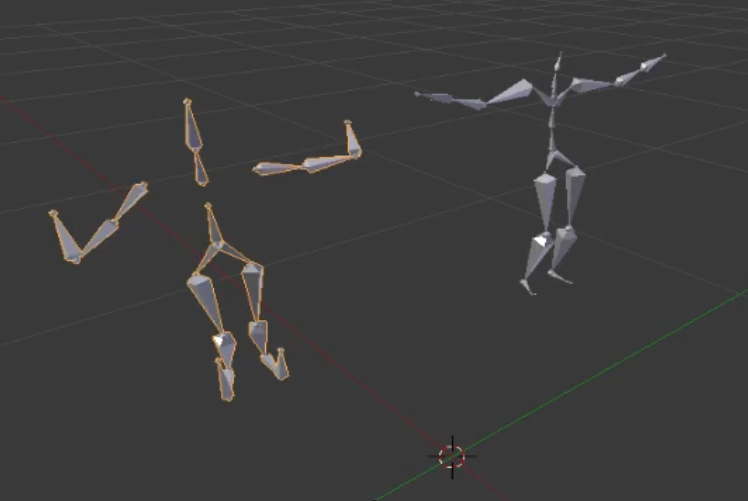
\includegraphics[width=1\linewidth, height=10cm]{images/retarget_wave.png}}
  \caption{Retargeted motion clip for hand wave skill}
  \label{fig:retarget_wave}
\end{figure}
\begin{figure} 
  \centering
  \href{https://youtu.be/wdyNuvNhy3o}{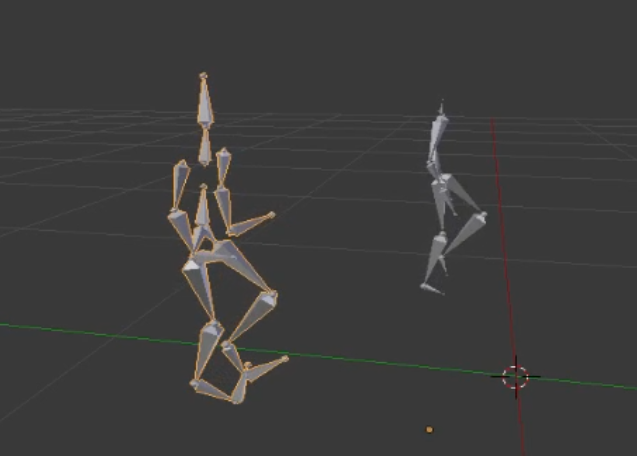
\includegraphics[width=1\linewidth, height=10cm]{images/retarget_wip.png}}
  \caption{Retargeted motion clip for walk in place skill}
  \label{fig:retarget_wip}
\end{figure}
\section{Training without Retargeting}
In the Training phase, initially to test the results of both phases independently we had manually created some motion clips which were free from retargeting errors. These include motion clips like hands opposite motion (in Fig \ref{fig:ho}), periodic squats motion (in Fig \ref{fig:squats}), manual partial walk in place motion (in Fig \ref{fig:mwip}). As you can see from these videos, that the robot is mimicking the motion to quite a good extent and further training will only improve these skills. All these skills have been trained using A3C code for around 50-60k episodes each using same reward function but with different state and action space. This space has been limited to only those joints whose orientation has non zero change involved in the motion clips (instead of all the original 22 joints). 

\section{Learning Curve}
Since 60k episodes take almost an entire day to learn, we implemented a mechanism to pause the learning process. This is done by saving current weights (as well as at some intermediate points) and then loading them to pick up where we left off. This not only helped us save the partially trained model in presence of runtime bugs but also helped us resume from particular checkpoints which were not corrupted. In the Fig \ref{fig:lc1}, we can see that in first 30k episodes, the learning curve (moving average of cumulative rewards v/s episodes) increased very slowly for almost 5k episodes and then picked up the pace to reach the maximum achievable value (which in this case was 120). In the Fig \ref{fig:lc2}, we can observe that in next 30k episodes, the growth in learning curve is slow as expected. Also, many times the moving average suddenly drops and grows fast again. Such events are marked by frequent spikes in both learning curves. This might be because of the agent trying out newer approaches/trajectories to see if there is any possibility of better cumulative rewards.

\begin{figure}[!b] 
  \centering
  \subfloat[Hands Opposite motion clip 1 - 30k episodes]{
    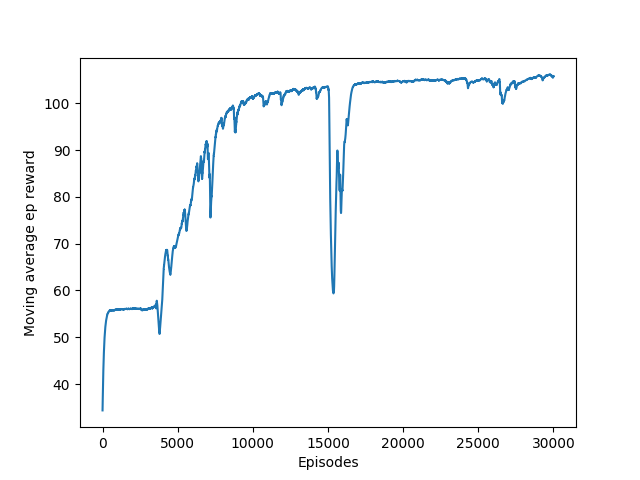
\includegraphics[width=1\linewidth, height=9.2cm]{images/lc_1.png}
    \label{fig:lc1}
  }
  \qquad
  \subfloat[Squats motion clip 30k -60k episodes]{
    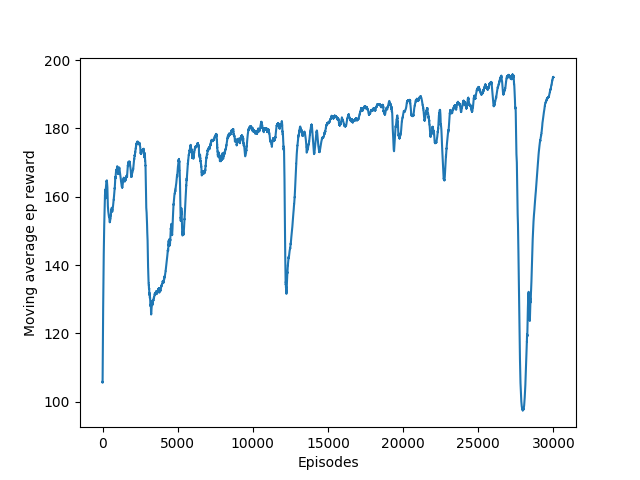
\includegraphics[width=1\linewidth, height=9.2cm]{images/lc_2.png}
    \label{fig:lc2}
  }
  \label{fig:x2}  
  \caption{Learning Curve for various motion clips in different stages}
\end{figure}

\begin{figure}[!ht]
    \centering
    \subfloat[Hands Opposite Skill]{
    	\href{https://youtu.be/lfb5rWUCuvw}{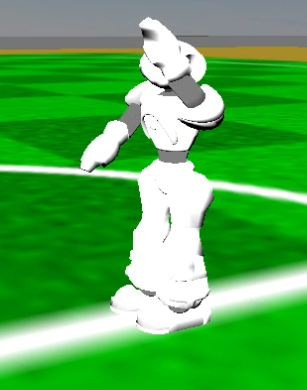
\includegraphics[width=0.3\linewidth, height=5cm,keepaspectratio]{images/ho.png}}
    	\label{fig:ho}
	}
    \qquad
    \subfloat[Squats Skill]{
    	\href{https://youtu.be/4LrHAHY2keg}{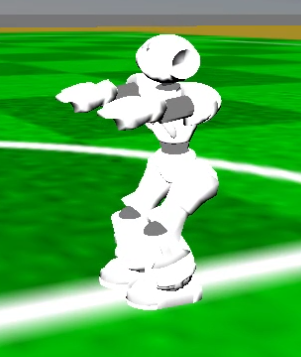
\includegraphics[width=0.3\linewidth, height=5cm,keepaspectratio]{images/squats.png}}
    	\label{fig:squats}
	}
    \qquad
    \subfloat[Walk in Place Skill]{
    	\href{https://youtu.be/yerCueG01oI}{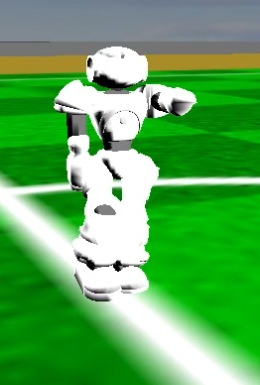
\includegraphics[width=0.3\linewidth, height=5cm,keepaspectratio]{images/mwip.png}}
    	\label{fig:mwip}
	}
    \label{fig:x1}
    \caption{Trained models for manually designed motion clips}
\end{figure}

\newpage
\section{Training with Retargeting}

After thorough testing, we also tried simulations over retargeted clips. These include hand wave motion (in Fig \ref{fig:wave}) and partial walk in place motion (in Fig \ref{fig:wip}). As you can see from the video of hand wave motion, that since the robot is well-balanced it can learn to mimic this motion quite well. However in case of walk in place motion, robot is not able to lift its leg as it has perhaps found a local minimum where lifting its leg only makes it fall (resulting in lower total reward) but partially copying the motion clip while maintaining balance gives higher cumulative reward. In this scenario, even though the retargeting seems smooth, learning to balance is a difficult task for our agent.

\begin{figure}[!ht]
    \centering
    \subfloat[Hand Wave Skill]{
    	\href{https://youtu.be/zeTAqHSJgxo}{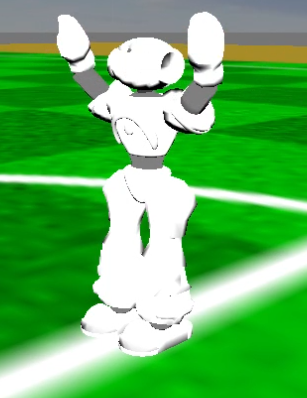
\includegraphics[width=0.4\linewidth, height=7cm]{images/wave.png}}
    	\label{fig:wave}
	}
    \qquad
    \subfloat[Walk in Place Skill]{
    	\href{https://youtu.be/IVX6FNjUJvo}{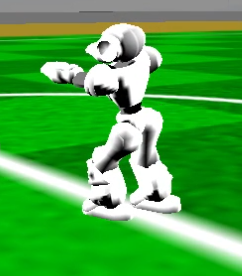
\includegraphics[width=0.4\linewidth, height=7cm]{images/wip.png}}
    	\label{fig:wip}
	}
    \qquad
    \label{fig:subfigname}
    \caption{Trained models for retargeted motion clips}
\end{figure}

\chapter{Conclusion and Future Work}

Clearly, our method shows that RL can be used to learn skills easily with the help of motion clip rewards.
For retargeted motions, the success is limited to motions where balancing is not required (like in hand wave motion) but for motions where we require balancing the robot struggles with handling balancing simultaneously with mimicking the motion clip. So if we could capture better motion clips tailor made for our nao agent we can surely make it able to not only walk but perform much more complex skills. 
\\\\
An important idea from [Xue Bin Peng et al. 2018] \cite{Peng:2018:DED:3197517.3201311} could possibly make this RL-motion clip reward system work. The idea is to start the simulation from not just the initial pose but also arbitrary in between poses. This would clearly help the robot learn later parts of simulation equally well. Currently, without this method learning longer (more than 3-4 sec) motion clips is difficult and requires a lot more episodes. We tried to implement this idea in our project but getting robot in stable initial pose is in itself a challenging task and would require a lot of manual effort and human insight. Extensions of this work could try to implement this random restart method and see if it actually improves the results or not.
\\\\
Furthermore, other target specific positional rewards could be used to get the robot to move along the ground(like described by [Xue Bin Peng et al. 2018]\cite{Peng:2018:DED:3197517.3201311}). After the agent learns a bunch of motions we can begin to teach it to switch between multiple motions at the right time which is very crucial during a soccer match.
\\\\
In conclusion, We tried an innovative and promising approach of combining animation with reinforcement learning applied to a completely different domain which can make soccer agent's behaviors more human-like and perhaps more effective. Unlike earlier approaches proposed, our approach doesn't require human intervention and creativity to optimize parameters for every particular type of behavior and agent can itself do what's best, provided we tune the reward functions in right manner once.

%****************************************************************
%                         Appendices                           
%****************************************************************
%% Additional, supporting material, such as codes, derivations, etc., can be placed in the appendix
% \appendix
% \chapter{Supporting Material}

%******************************************************************
%                         Bibliography or References          
%******************************************************************  
\bibliography{mylit}     

%*******************************************************************
%                         List of publications               
%******************************************************************
% %%%
\listofpublications


\noindent Put your publications from the thesis here. The packages \texttt{multibib} or \texttt{bibtopic} or \texttt{biblatex} or enumerate environment or thebibliography environment etc. can be used to handle multiple different bibliographies in the document.








%%======================================================================
%%% Local Variables: 
%%% mode: latex
%%% TeX-master: "../mainrep"
%%% End: 







            
          

%*******************************************************************
%                        About author                    
%*******************************************************************
% \colophon % remove this command while using this file.

% GAME OVER
%*******************************************************************
\end{document}

%%% Local Variables: 
%%% mode: latex
%%% TeX-master: t
%%% End: 
